\documentclass[aspectratio=169]{beamer}
\usepackage[utf8]{inputenc}
\usepackage[T1]{fontenc}
\usepackage[french]{babel}
\usepackage{graphicx}
\usepackage{pgfpages}

\usetheme{Boadilla}
% \setbeameroption{show notes on second screen=right}

\title{Leçon 3 : Logique du Premier Ordre}
\subtitle{Quantificateurs et Égalité dans Rocq}
\author{Logique et Fondements de l'Informatique}
\date{Année 2026}

\begin{document}

\begin{frame}
  \titlepage
  \note{Bonjour à tous. Aujourd'hui nous entamons la troisième leçon. Jusqu'à présent, nous étions cantonnés à la logique propositionnelle, où les atomes étaient de simples variables A, B, C invisibles de l'intérieur. Aujourd'hui, on ouvre le capot et on regarde les individus qui peuplent nos mondes mathématiques avec la logique des prédicats.}
\end{frame}

\begin{frame}{Les Prédicats comme Fonctions}
  \begin{columns}
    \begin{column}{0.5\textwidth}
      \textbf{D'une proposition à une propriété:}
      \begin{itemize}
        \item Avant: $A : \text{Prop}$
          \pause
        \item Maintenant: Type domaine $T$
        \item Prédicat: $P : T \to \text{Prop}$
          \pause
        \item La propriété est testée sur un individu $x$.
      \end{itemize}
    \end{column}
    \begin{column}{0.5\textwidth}
      \begin{center}
        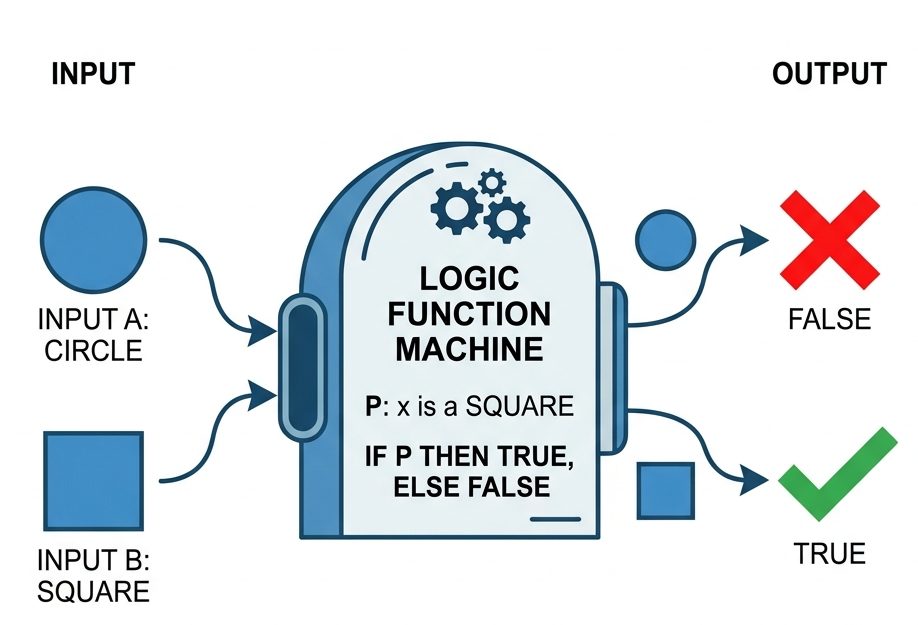
\includegraphics[width=0.95\textwidth]{images/predicat.png}
      \end{center}
    \end{column}
  \end{columns}
  \note{Dans Rocq, et par l'inspiration originale de Alonzo Church, un prédicat n'est rien d'autre qu'une fonction. Elle prend un individu et recrache une proposition. C'est une vision très élégante où les $\lambda$-termes servent à la fois pour les preuves et pour les prédicats eux-mêmes. Attention cependant, dès qu'on touche à un univers de type, on doit faire attention au fameux paradoxe de Girard, qui est l'analogue du paradoxe de Russell pour les types de types. Heureusement l'architecture de Rocq gère ça via les univers.}
\end{frame}

\begin{frame}{Le Quantificateur Universel ($\forall$)}
  \begin{itemize}
    \item Noté \texttt{forall x : T, P x} en Rocq.
      \pause
    \item Informatiquement : un \textbf{type dépendant}.
      \pause
    \item C'est une fonction qui à tout $x$ associe une \emph{preuve} de $P(x)$.
      \pause
    \item L'implication \texttt{A -> B} est juste un cas particulier !
  \end{itemize}
  \note{Il est crucial de comprendre que `A -> B` et `forall x : A, ...` sont manipulés exactement par les mêmes tactiques. Une implication c'est juste un pour tout qui ignore l'individu en argument ! C'est la beauté de la correspondance de Curry-Howard.}
\end{frame}

\begin{frame}{Le Quantificateur Existentiel ($\exists$)}
  \begin{itemize}
    \item Noté \texttt{exists x : T, P x} en Rocq.
      \pause
    \item Constructivisme exige : il faut trouver \emph{le témoin}.
      \pause
    \item Preuve = Paire $(t, \pi)$
      \begin{itemize}
        \item $t : T$ (le témoin)
        \item $\pi : P(t)$ (la justification)
      \end{itemize}
      \pause
    \item Mêmes mécanismes que la conjonction \texttt{/\textbackslash}.
  \end{itemize}
  \note{En constructivisme strict, dire "Il existe", c'est être capable de montrer "Voici la chose". C'est pour ça qu'on a besoin d'exhiber le témoin physiquement avec la tactique `exists`. Et quand on a une hypothèse existentielle, `destruct` nous la coupe en deux: le témoin, et sa preuve.}
\end{frame}

\begin{frame}{L'Égalité Propositionnelle (=)}
  \begin{columns}
    \begin{column}{0.5\textwidth}
      \textbf{Leibniz \& Substitution}
      \begin{itemize}
        \item $x = y$ est une proposition.
          \pause
        \item Indiscernabilité conceptuelle.
          \pause
        \item Tactique clé : \texttt{rewrite}
      \end{itemize}
    \end{column}
    \begin{column}{0.5\textwidth}
      \begin{center}
        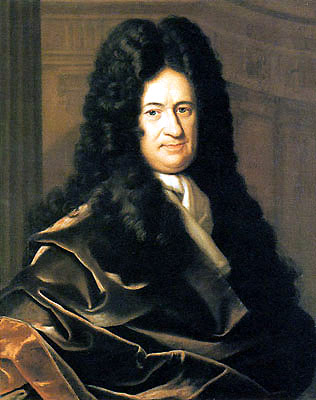
\includegraphics[height=0.6\textheight,keepaspectratio]{images/leibniz.jpg}
      \end{center}
    \end{column}
  \end{columns}
  \note{Venons-en à l'égalité. L'outil principal de l'algèbre à l'école, c'est de substituer y à la place de x dès qu'on sait que x = y. Rocq fait ça avec `rewrite`. Remarquez que conceptuellement, cela invoque fondamentalement le principe de l'indiscernabilité des identiques de Leibniz. On s'en sert ici de manière utilitaire, en supposant que la plupart d'entre vous le maitrisent déjà un peu, et on justifiera la théorie profonde derrière ce principe la semaine prochaine.}
\end{frame}

\begin{frame}{Égalité Définitionnelle ($\equiv$) vs Propositionnelle (=)}
  \begin{itemize}
    \item Propositionnelle : Exige une \emph{preuve} manuelle (\texttt{rewrite}, lemmes).
      \pause
    \item Définitionnelle : La \emph{machine} évalue le code pour vous.
    \item Exemples :
      \begin{itemize}
        \item $2 + 2 \equiv 4$ (calcul)
        \item \texttt{doubler 2} $\equiv 4$ (expansion/$\beta$-réduction)
      \end{itemize}
      \pause
    \item Tactique : \texttt{reflexivity} triomphe sans effort sur $\equiv$.
  \end{itemize}
  \note{C'est la chose la plus déroutante mais la plus puissante pour les nouveaux venus. Contrairement à la logique sur papier où vous devez justifier chaque étape de calcul mentalement, Rocq embarque l'exécution du code dans la théorie logique. La tactique reflexivity dit non seulement x=x, mais aussi que tout terme qui s'évalue à x est égal à x ! Ca permet des preuves magiques pour les calculs triviaux.}
\end{frame}

\begin{frame}{Synthèse}
  \begin{itemize}
    \item \texttt{forall} $\sim$ fonctions ($\rightarrow$) / tactique \texttt{intro}
    \item \texttt{exists} $\sim$ paires ($\land$) / tactique \texttt{destruct}
    \item \texttt{rewrite} pour la substitution équationnelle
    \item \texttt{reflexivity} pour laisser l'ordinateur calculer
  \end{itemize}
  \note{On va maintenant passer au Live Coding sur jsCoq. Je vais vous montrer tout ça en action sur de petits exemples avant de vous laisser attaquer le TP de cette leçon 3.}
\end{frame}

\end{document}
